% comparison results (number of nodes expanded, time, etc.) for the path finding problemsas the Pacman plans and replans in the environment; figures are helpful here. 


\section{Evaluation}\label{sec:eval}
	\subsection{Configuration and Metrics}
    The four metrics used to measure the performance of the search algorithms were path length, nodes expanded, memory usage, and running time. Path length describes the length of the final path that Pacman took in order to find the goal state. This path is the same path that is visualized in the Pacman environment. Nodes expanded measures the number of nodes that needed to be expanded, i.e. popped from the priority queue in order to complete the search. The nodes expanded metric is linked to both time and space complexity. This is because the more nodes expanded, the longer the search will take. Also, the more nodes expanded, the deeper the queue, and the more space is needed to store those nodes in the queue. Memory use describes the maximum amount of memory used at a given point in time (in MB) by the Pacman Python process. The memory usage was  captured using the $\texttt{valgrind}$ utility. Running time captures the effective amount of time was needed to guide the agent to the goal location. The runtime was captures by using the linux $\texttt{time}$ command. 
    
    All of these metrics were measured as a function of maze size, i.e. the effective area of a the Pacman maze in test. Note that there is not a direct linear relationship between maze size and search complexity, since the maze size does not capture other factors, such as complexity or wall count. However, the maze size is correlated with search complexity and in general, the larger the maze size, the more complex the search problem.
    
    A* search was also included as a baseline comparison. Note that the A* algorithm has a totally observable environment, whereas the other three algorithms only have a partially observable environment, namely the 4 adjacent cells in the Pacman environment.
    
    The experiments were run using a machine with 8-core Intel i5 1.6 GHz processor and 12 GB of RAM. 
    
    \subsection{Experiments and Discussion}
    
    We executed and collected metrics for each search algorithm against four different environments: the pre-defined tiny (7x7), small (22x10), medium (36x18), and big (37x37) mazes of the Pacman domain. Results were tabulated, graphed, and the decision was made to switch the units to logarithmic for better visibility. Each approach was executed once, as the pathfinding process for these algorithms is deterministic.
    
    

	For all algorithms, the path lengths increase with respect to the maze size (see Figure 1). The A* algorithm has the best performance as expected, followed by NRA* and D* Lite, and finally be LPA*. The explanation for the low performance of LPA* is that it continually backtracks to the intersection point, which contributes to the path cost.

\begin{figure}[t]
	\centering
	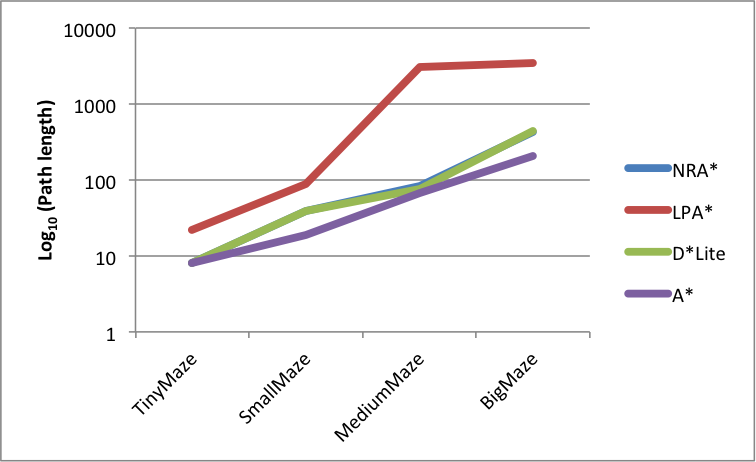
\includegraphics[width=7cm]{PathLength.png}
	\caption{Path Length v. Maze Size}
	\label{fig:1}
\end{figure}

	\begin{figure}[t]
		\centering
		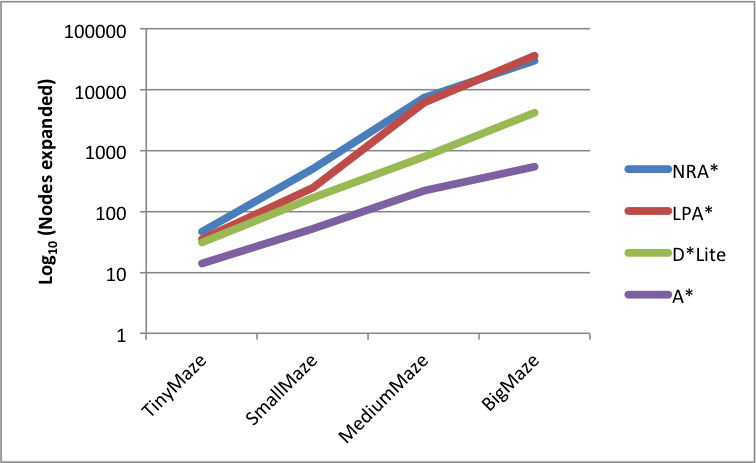
\includegraphics[width=7cm]{NodesExpanded.png}
		\caption{Nodes Expanded v. Maze Size}
		\label{fig:2}
	\end{figure}


	\vspace{-0mm}
	For all algorithms, the number of nodes expanded increases with respect to the maze size (see Figure 2). The order of performance from best to worst is as expected: A*, D* Lite, LPA*, and NRA*. The low performance for NRA* can be explained by the re-planning nature of its implementation. Every time it hits a wall on its expected path, it re-plans from scratch, i.e. the nodes explored and nodes in its fringe are not carried over when calling A* again. This is what LPA* and D* Lite aim to avoid. 

	\begin{figure}[t]
		\centering
		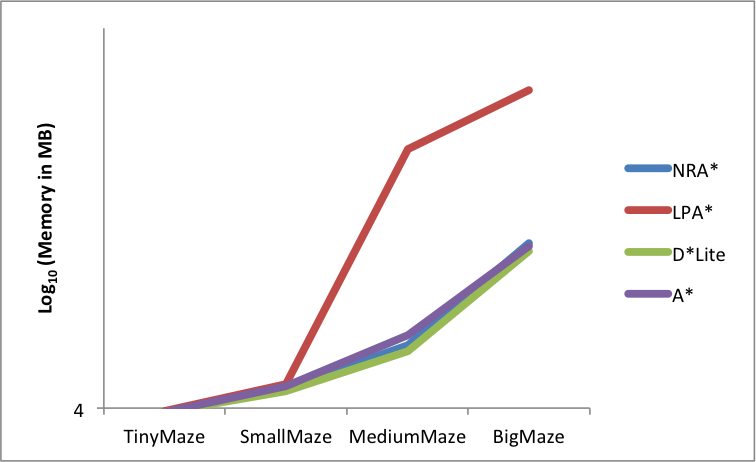
\includegraphics[width=7cm]{Memory.png}
		\caption{Memory v. Maze Size}
		\label{fig:3}
	\end{figure}

	For all algorithms, the amount of memory increases with respect to the maze size (see Figure 3). The order of performance from best to worst is: D* Lite, NRA*, A*, and finally LPA*. D* Lite slightly out-performs all other algorithms because of specific measures it takes to only re-evaluate those nodes that will have an affect on the final path. Again, the low performance of LPA* is due to the backtracking nature. This is somewhat counterintutive, as A* and NRA* do not maintain in-memory structures of the same complexity as the other two; we conclude that the memory usage is likely dominated by the Pacman domain implementation itself, as memory usage and path length are highly correlated.

	\begin{figure}[t]
		\centering
		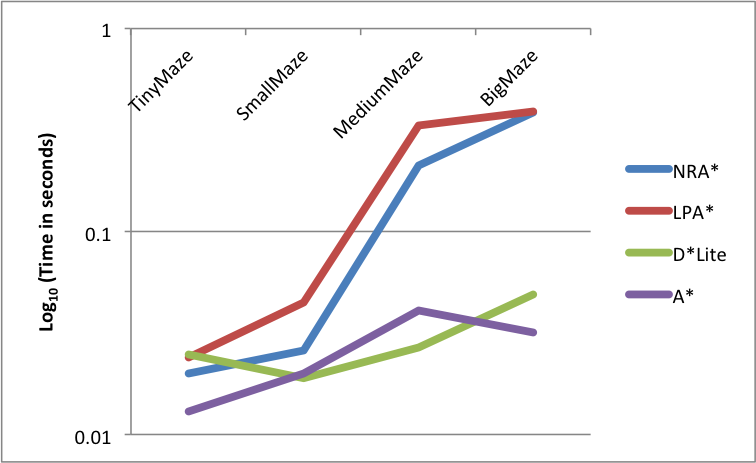
\includegraphics[width=7cm]{Time.png}
		\caption{Runtime v. Maze Size}
		\label{fig:4}
	\end{figure}

	For all algorithms, the runtime  increases with respect to the maze size (see Figure 4). A* and D* Lite are the best performers, with alternating dominance. Interestingly, this shows that even if the agent has partially observable environment information, it can potentially perform just as fast or faster than an agent with total observability of the environment, using the right strategy, namely D* Lite in this case. This is because A* follows a ``perfectionist" strategy, and finding the optimal route may take computational longer than the ``good enough" route found by D* Lite. These are followed by NRA* and finally LPA*. These two struggle due to their backtracking and re-planning nature, respectively.
	
	Overall, D* Lite is the most competitive of the re-planning algorithms, especially in computation time. LPA* was not as competitive as we expected, primarily due to the backtracking process necessitated by the Pacman domain integration.